
\subsection{Question Group 4 - Supply Chain Standalone Points of Improvement and Blockchain points of Applicability and Improvement for Supply Chain}
\label{sec-survey-improvement-functionalities}

The first goal for this part of the survey is to find out the points of improvement for supply chain. What is being questioned are not the issues of the supply chain themselves, which were already asked, but what parts of supply chain, even though they may already work well, could work even better.

The second goal is to find out more about the requirements that an information system must have to satisfy the needs of SCM. This includes ranking the functionalities of an information system for their importance. Many of these functionalities probably relate to the points of improvement found here, as well as to the supply chain issues described in Section~\ref{sec-supplychainissues}.

%Problema: há varios graficos para mostrar, mas alguns deles, como o da figura 6.1, têm varias (7 a 8) distribuições para mostrar, onde cada uma delas tem os seus valores das metricas.

%2 EM 1
%GRAFICOS DOS SUPPLY CHAIN IMPROVEMENT ASPECTS


For the sake of simplifying the ranking process for both the \textit{"points of improvement"} and \textit{"functionalities of an information system"}, a division into groups of importance shall be done according to the observed results. The importance scale went from 1 to 5, but most of the mean scores were between 3 and 4.5. 

Therefore, the following classification for the lists of results will be adopted: 

\begin{itemize}
    \item \textbf{Mean 	$\geq$ 4} - High priority or importance
    \item \textbf{3.5 $\leq$ Mean $<$ 4} - Medium importance 
    \item \textbf{Mean $<$ 3.5} - Low importance
\end{itemize}

\subsection*{1 - Rank the importance of some aspects which Supply Chains aim to improve.}
 
%Dividir em mais imagens?
%\todo{fcorreia: sim, está muito pequeno para se ler assim. talvez quatro ou cinco destes gráficos lado a lado fiquem ok...}

\begin{figure}[h]
\centering
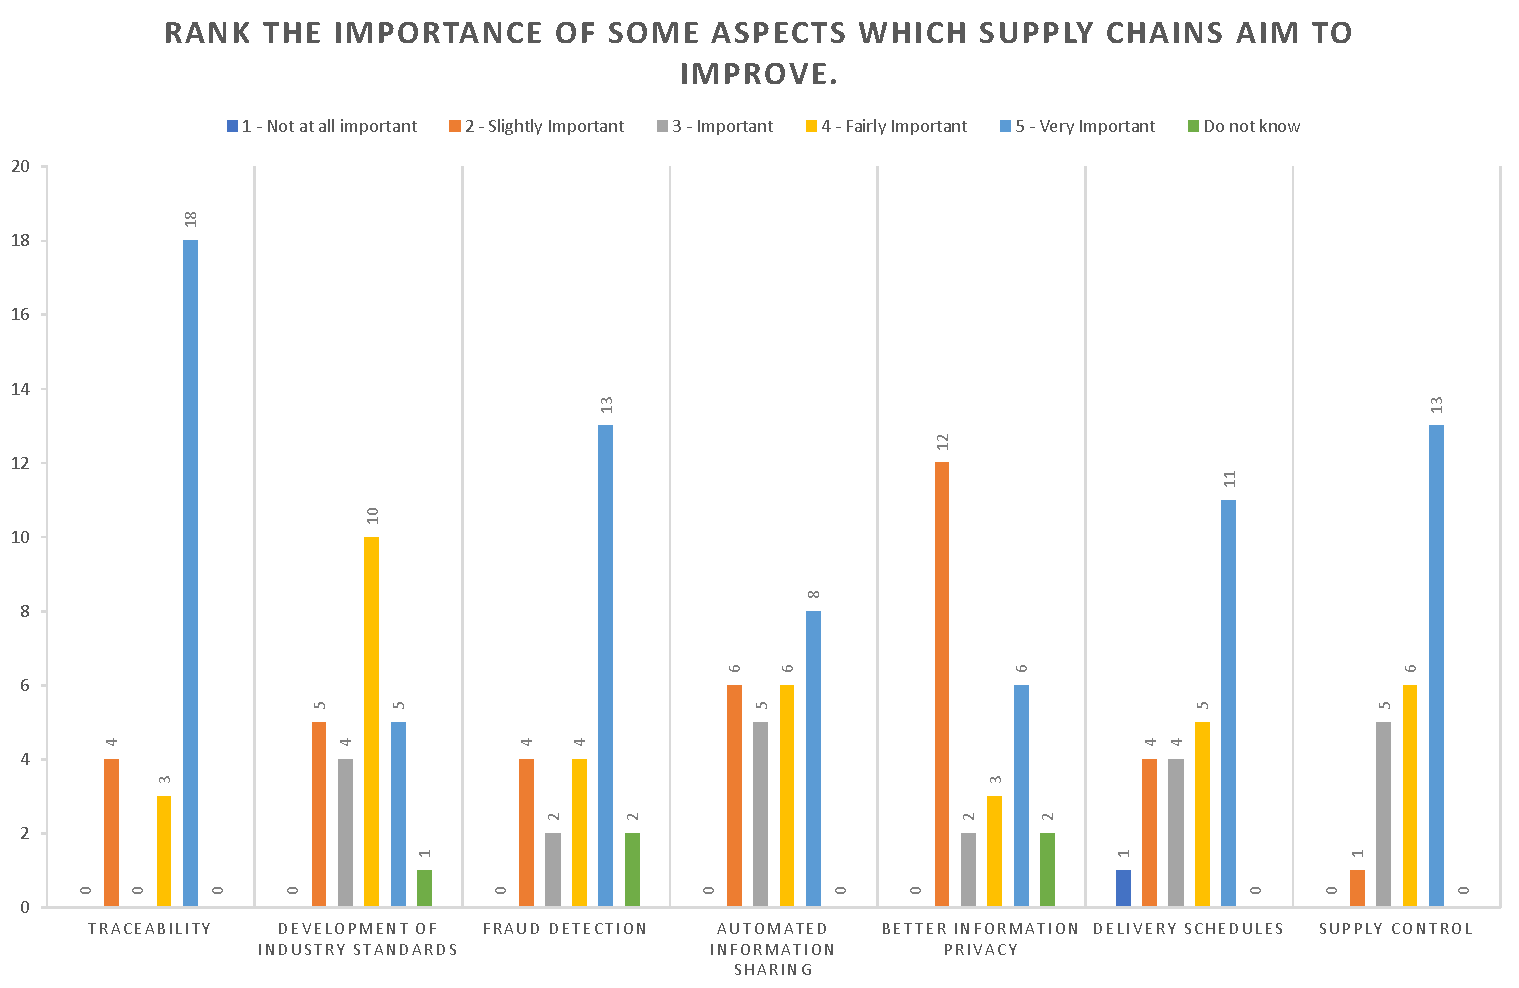
\includegraphics[scale=0.60]{media/survey_group4/importance_SC_improvement_points.pdf}
\caption{Question: "Rank the importance of some aspects which Supply Chains aim to improve."}
\label{fig:importance_SC_improvement_points}
\end{figure}

%%%%%%%% TABLE BEGIN %%%%%%%%%

\begin{table}[h]
\centering
\caption{Question results metrics for the question to rank the importance of improvement aspects of the supply chain.}
\label{table:metrics-importance-improvement-sc}
\resizebox{\textwidth}{!}{
\begin{tabular}{l|l|l|l|l|l|l|}
\cline{2-7}
                                                                                                    & Mode & Median & Mean   & \begin{tabular}[c]{@{}l@{}}Standard\\ Deviation\end{tabular} & Range & Skewness \\ \hline
\multicolumn{1}{|l|}{Traceability}                                                                  & 5    & 5      & 4,40  & 1,12                                                       & 3     & -1,67  \\ \hline
\multicolumn{1}{|l|}{\begin{tabular}[c]{@{}l@{}}Development\\ of Industry\\ Standards\end{tabular}} & 4    & 4      & 3,63 & 1,06                                                       & 3     & -0,36  \\ \hline
\multicolumn{1}{|l|}{\begin{tabular}[c]{@{}l@{}}Fraud\\ Detection\end{tabular}}                     & 5    & 5      & 4,13 & 1,18                                                       & 3     & -1,00  \\ \hline
\multicolumn{1}{|l|}{\begin{tabular}[c]{@{}l@{}}Automated\\ Information \\ Sharing\end{tabular}}    & 5    & 4      & 3,64 & 1,19                                                       & 3     & -0,200  \\ \hline
\multicolumn{1}{|l|}{\begin{tabular}[c]{@{}l@{}}Better\\ Information\\ privacy\end{tabular}}        & 2    & 2      & 3,13 & 1,32                                                       & 3     & 0,51   \\ \hline
\multicolumn{1}{|l|}{\begin{tabular}[c]{@{}l@{}}Delivery\\ Schedules\end{tabular}}                  & 5    & 4      & 3,84 & 1,28                                                       & 4     & -0,71  \\ \hline
\multicolumn{1}{|l|}{Supply Control}                                                                & 5    & 5      & 4,24 & 0,926                                                       & 3     & -0,87  \\ \hline
\end{tabular}
}
\end{table}

%%%%%%%% TABLE END %%%%%%%%%%%%%%%%

In this category, we can see the results on Table~\ref{table:metrics-importance-improvement-sc}. Pretty much all the options had a range of 3 and deviations close to 1, which is to be expected. Traceability had the highest skew value, as there seemed to be some dissent, as a few outlier values pushed the mean to be lower than the median. However, it still rated the highest, by importance. 

The importance ranking described as before follows below:

\begin{enumerate}
    \item \textbf{High importance} - "Traceability", "Supply Control", "Fraud Detection";
    \item \textbf{Medium importance} - "Delivery Schedules", "Automated Information Sharing", "Development of Industry Standards"
    \item \textbf{Low importance} - "Better Information Privacy"
\end{enumerate}

\par \textbf{Conclusions: }
%Points of failure from before: traceability, inventory management is ESSENTIAL
\begin{itemize}

\item High Importance - It had already been concluded from the previous set of questions in~\ref{sec-supplychainissues} that inventory management was an essential discipline to SCM, so it was expected that \textit{Supply Control} would be rated highly as a point of improvement, which it did. The same can be said about \textit{Traceability}: it was expected to rank highly, since it is related to both quality assurance and availability of information, two other issues that were validated in the previous set of questions. At the same time, \textit{Fraud Detection} was also highly ranked, which can be explained by its relation to traceability and quality compliance and control. \textbf{Traceability helps to avoid fraud and, at the same time, fraud detection also relates to quality control and compliance, since avoiding fraud is all about making sure that the products circulating the supply chain are authentic and have good quality.} With this in mind, it is only natural that Fraud Detection is considered important, together with traceability.

\textbf{In conclusion, the 3 most important items are traceability, supply control and fraud detection, with supply control and fraud detection directly depending on the traceability, which makes traceability probably the most important point of improvement in the supply chain.}

\item Medium Importance - From the items that got rated as medium importance, 2 of them relate to synchronization improvement: \textit{Automated Information Sharing} and \textit{Development of Industry Standard}. The last point, \textit{Delivery Schedules} also relates to Supply Control, though it is less generic.

\textbf{In conclusion, though system synchronization is not as important as traceability or some of the other items that depend on traceability, it is still a welcome improvement which comes in second place to the others.}


\item Low Importance - Finally, the lowest ranking item was \textit{Better Information Privacy}. This comes as a surprise, since security was a big focus on the background research for supply chain management. 

\textbf{The conclusion we can take from this item being rated the lowest, is that it might be a concern that the current systems already take care of, therefore it does not have much space for improvement.}
\end{itemize}


%2 EM 1https://www.overleaf.com/13104200fnmytzmhwtck#
%GRAFICOS DOS BLOCKCHAIN POINTS OF APPLICABILITY
\subsection*{2 - Rank the importance of the following functionalities for an information system that stores or processes data pertaining to a Supply Chain}

\begin{figure}[h]
\centering
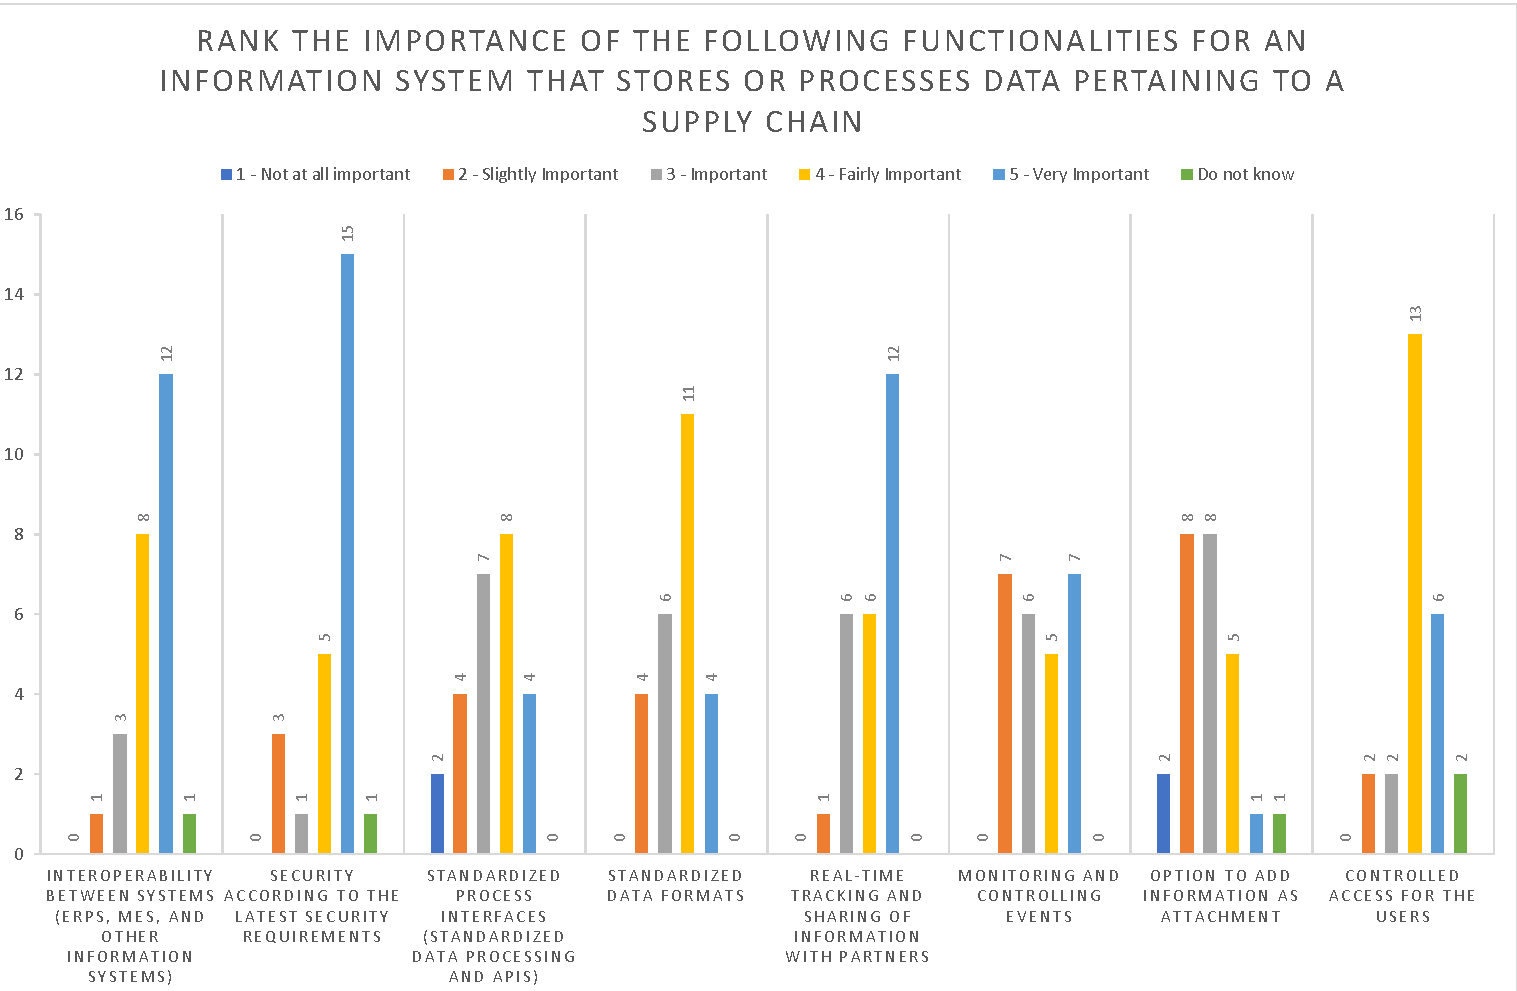
\includegraphics[scale=0.60]{media/survey_group4/importance_SC_info_systems.pdf}
\caption{Question: "Rank the importance of some functionalities in a supply chain based information system."}
\label{fig:importance_SC_info_systems}
\end{figure}

%%%% TABLE START %%%%%%%%%%

\begin{table}[h]
\centering
\caption{Question results metrics for the question to rank the importance of functionalities in an information system for supply chain.}
\label{table:metrics-importance-info-systems}
\resizebox{\textwidth}{!}{
\begin{tabular}{l|c|c|c|c|c|c|}
\cline{2-7}
                                                                                                                                                & \multicolumn{1}{l|}{Mode} & \multicolumn{1}{l|}{Median} & \multicolumn{1}{l|}{Mean} & \multicolumn{1}{l|}{\begin{tabular}[c]{@{}l@{}}Standard\\  Deviation\end{tabular}} & \multicolumn{1}{l|}{Range} & \multicolumn{1}{l|}{Skewness} \\ \hline
\multicolumn{1}{|l|}{\begin{tabular}[c]{@{}l@{}}Interoperability Between \\ Systems (ERPs, MES, \\ and other information systems)\end{tabular}} & 5                         & 4,5                         & 4,29                    & 0,86                                                                             & 3                          & -1,08                       \\ \hline
\multicolumn{1}{|l|}{\begin{tabular}[c]{@{}l@{}}Security according to the\\  latest security requirements \end{tabular}}                                               & 5                         & 5                           & 4,33                    & 1,05                                                                             & 3                          & -1,49                       \\ \hline
\multicolumn{1}{|l|}{\begin{tabular}[c]{@{}l@{}}Standardized Process Interfaces \\ (Data Processing and APIs)\end{tabular}}                     & 4                         & 3                           & 3,32                    & 1,18                                                                            & 4                          & -0,36                       \\ \hline
\multicolumn{1}{|l|}{Standardized Data Formats}                                                                                                 & 4                         & 4                           & 3,60                    & 0,96                                                                             & 3                          & -0,31                       \\ \hline
\multicolumn{1}{|l|}{\begin{tabular}[c]{@{}l@{}}Real-time tracking and sharing \\ of information with partners\end{tabular}}                    & 5                         & 4                           & 4,16                    & 0,94                                                                             & 3                          & -0,67                       \\ \hline
\multicolumn{1}{|l|}{Monitoring and controlling events}                                                                                         & 5                         & 3                           & 3,48                    & 1,19                                                                             & 3                          & 0,05                       \\ \hline
\multicolumn{1}{|l|}{\begin{tabular}[c]{@{}l@{}}Option to add information \\ as attachment\end{tabular}}                                        & 2                         & 3                           & 2,79                    & 1,02                                                                             & 4                          & 0,19                        \\ \hline
\multicolumn{1}{|l|}{Controlled access for the users}                                                                                           & 4                         & 4                           & 4                         & 0,85                                                                             & 3                          & -0,96                       \\ \hline
\end{tabular}
}
\end{table}


Results for this question are found in Figure~\ref{fig:importance_SC_info_systems}, and the analysis metrics are in Table~\ref{table:metrics-importance-info-systems} the range of answers is pretty much 3 for all options but 2 of them. The mean and median of the items are also a close approximation of each other, which happens because the skew in most cases is  not very high (only for the Interoperability and Security items was it higher than 1). The skew is highest on the items that also had the highest mean. This happens because, even though these items are the most popular, there are always a few answers from people who disagree. However, this is to be ignored, given the low deviation and given that the median and mean are very close to each other in every case. Therefore, the mean can still be used here to classify the importance.

The importance ranking described as before follows below:

\begin{enumerate}
    \item \textbf{High importance} - "Security according to the latest requirements", "Interoperability Between Systems", "Real-time tracking and sharing of information", "Controlled access for the users";
    \item \textbf{Medium importance} - "Standardized Data Formats"
    \item \textbf{Low importance} - "Monitoring and controlling events", "Standardized Process Interfaces", "Option to add information as attachment"
\end{enumerate}

\par \textbf{Conclusions: }
\begin{itemize}

    \item 2 of the high importance items actually relate to security, namely access control and following security requirements. This contrasts with the point of improvement from the previous set of questions \textit{"Better information privacy"}, which was rated the lowest in relative importance. There seems to be a disparity between the importance of the functionality and the importance of the improvement, which might mean that the functionality is important but already good enough as it is.
    
    \textbf{The conclusion we can take is that keeping security up to date still seems to be considered important, but on aspects other than privacy (which is already fulfilled) such as access control, which relates to authorization and authentication.}

    \item The other 2 high importance functionalities were about interoperability between systems, and tracking and sharing information. Tracking and sharing information relates to traceability and information synchronization, while interoperability relates only to synchronization.

    \textbf{Though these points, which relate to synchronization scored high as a functionality, the points of improvement they relate to only scored as medium in the previous sections, namely \textit{"Automated Information Sharing"} and \textit{"Development of Industry Standards"}. Thus, integrating the information is seen as an important aspect to have,but not one that needs improvement over the current status.}

\item Most of the items rated as having medium or low importance do not necessarily stand out nor do they have important conclusions to be taken. The one thing that stands out is that \textit{"Monitoring and controlling events"} rated as a low importance functionality, even though traceability rated high as a point of improvement, which does not make a lot of sense, since traceability also means having the means to monitor what is happening.


\end{itemize}

%%%% TABLE END %%%%%%%%%%

\subsection*{3 - Blockchain applicability to the supply chain}
 
%CHANGE IMAGES TO THE 2 GRAPHICS ABOUT USE CASES OF BC+SC AND BENEFITS OF BC+SC

The final important group of questions featured 2 questions about the viability of applying blockchain to the supply chain. The first question asked people which use cases they thought were the best for applying blockchain to the supply chain and respondents could select a maximum of 3 options (including "None" or "Do not know").

\begin{figure}[h]
    %\makebox[2pt]{}

	\resfig{survey_group4/blockchain_usecases_sc}{Blockchain use cases for the supply chain}
    \resfig{survey_group4/blockchain_application_benefits}{Blockchain benefits for the supply chain}
    
      \caption{Question: Blockchain use cases and benefits for the supply chain.}
    \label{fig:group4_graphics}
\end{figure}

\textbf{Starting with the analysis of the first question}:
\begin{itemize}
    \item \textbf{Financial transactions was, by far, the most popular choice.} The respondents look at blockchain as a way to move money as an asset, more than a tool to manage the goods themselves, since traditional systems only deal with data and the money is dealt with by third parties (banks). It makes sense that \textbf{the second most voted choice is Contract Enforcement.} As per the background research and state of the art, it was pointed out that some of the applications already enforce payments through contracts, when the goods are delivered,for instance, without the need of a third party (thus reducing fees). Financial transactions and contract management go hand in hand. 
     
    \item With the same number of votes, \textbf{also in second place, is "regulatory compliance and auditing"}. Regulatory compliance is a term also related to contracts enforcement. Contracts are used to establish mandatory rules which are automatically enforced according to the conditions of the system (for instance, enforce that the food transported in a truck never goes over a certain temperature value). \textbf{However, an important point to note is that regulatory compliance and auditing are made possible through the traceability characteristic of blockchain, which allows for products and processes to be thoroughly verified. This means that traceability is a highly sought after application of blockchain.}
    \item "Secure data storage" was also a highly voted option. Security is an important focus in information systems, so this should be taken into account when building the proof-of-concept. In the previous set of questions, "access control" and "security according to the latest requirements" were also features that stood out, so \textbf{it is not a surprise that secure data storage is seen as one of the main advantages of blockchain, since it boasts of being cryptographically secure, having immutability by design and an easy to implement access control.}. 

\end{itemize}

The proof-of-concept has to not only take these use cases into account as the main applications, but also implement (or make possible the implementation of) the most important features of information systems previously analyzed, which makes the second question complementary of the first one.

\textbf{For the second question, there is an analysis of the benefits that blockchain can bring to the supply chain, according to the respondents}:

\begin{itemize}
    \item The three most voted items were: \textit{"Better transaction integrity and visibility"}, \textit{"Reduction of risks (fraud/tampering/information leaks)"} and \textit{"Stronger working relationships with partners"}.

    The first two items were expected to rank high. They directly relate to the security and traceability, points of improvement already discussed - traceability makes it possible to view the records to make sure nothing suspicious is going on, and the security and immutability of the information makes it impossible to tamper with the data.
    
    The third point, "Stronger working relationships with partners", however, is interesting to see being chosen a high ranked benefit. The concept of strong relationships with partners is linked to  the concept of \textbf{internal supply chain trust}, which was already introduced in~\ref{sec:advantes-blockchain}. The ability for partners to trust each other is what makes the supply chain possible and efficient to the standards of today. It seems that the professionals really do think of blockchain as a tool to improve this internal trust.
    
    The selection of these 3 items as the most voted does not seem to be a coincidence. \textbf{Blockchain can be used as a source of truth for the supply chain and this leads to the side benefits of internal trust, better relationships with the partners, less fraud, less tampering, less leaks, among other benefits, all made possible because of the main characteristics: security and traceability.}
\end{itemize}

\subsection*{Conclusions from Question Group 4}

This was the most important group of questions in that it provides direct information as to which functionalities the proposed system design should possess and implement. At the same time, these functionalities can be related to the points of improvement found, as well as to the issues validated in the previous groups of questions.

\begin{itemize}
    \item From question group 3, some issues in the supply chain were validated: \textbf{inventory management}, \textbf{quality assurance} and \textbf{getting accurate and timely data}. On this group, the main points of improvement were found to focus on: \textbf{traceability}, \textbf{supply control}, \textbf{fraud detection} and \textbf{synchronization}. In a generalized way, the common links to both issues and points of improvement seem to be: \textbf{security}, \textbf{traceability} and \textbf{synchronization}, effectively validating the initial concerns from the problem statement.
    \item Another important conclusion to take from this set of questions are the features to include in the design for the blockchain system. These include the \textit{\textbf{"Blockchain only features"}}, functionalities implemented in an unique to the blockchain, as well as the standard \textit{\textbf{"Information system features"}}, which are the features that were found to be the most important to information systems in a supply chain.
    \item By order of importance, the blockchain features are:
    \begin{itemize}
        \item Financial transactions.
        \item Some form of regulatory auditing.
        \item Enforceable contracts (smart contract functionality).
        \item Secure data storage.
        \item Asset management.
    \end{itemize}
    \item By order of importance, the most important information system requirements are:
    \begin{itemize}
        \item Security according to the latest requirements.
        \item Interoperability between systems.
        \item Real-time tracking and sharing of information with partners.
        \item Controlled access for the users.
    \end{itemize}
\end{itemize}











